\begin{figure}
    \centering
    \begin{subfigure}{0.45\textwidth}
        \centering
        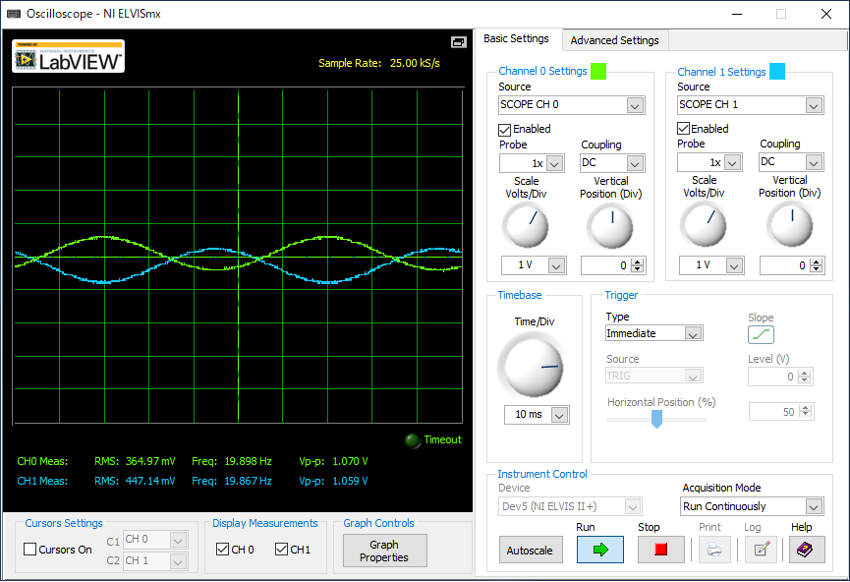
\includegraphics[width=0.8\linewidth]{src/figures/exp7/sum-0.png}
        \subcaption{VPS: \SI{0}{V}}\label{fig:exp7-raw-0}
    \end{subfigure}
    \begin{subfigure}{0.45\textwidth}
        \centering
        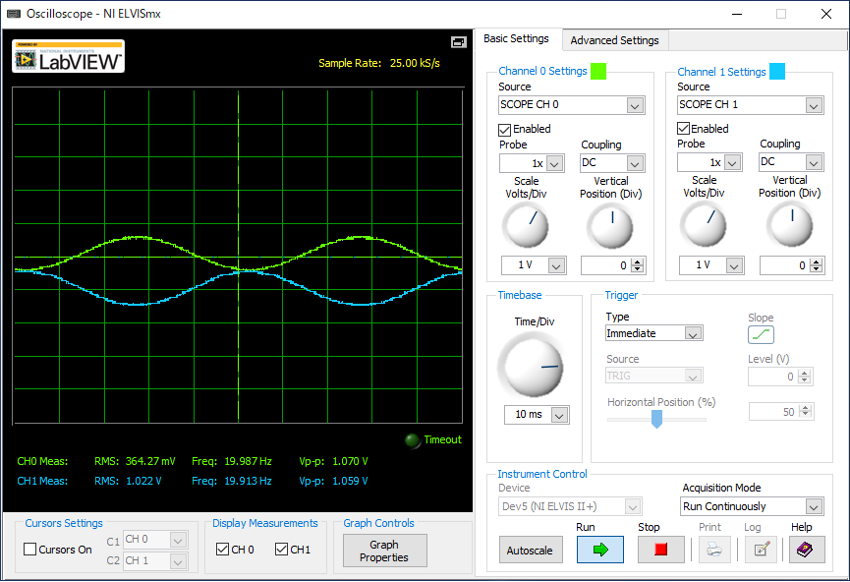
\includegraphics[width=0.8\linewidth]{src/figures/exp7/sum-1.png}
        \subcaption{VPS: \SI{1}{V}}\label{fig:exp7-raw-1}
    \end{subfigure}
    \begin{subfigure}{0.45\textwidth}
        \centering
        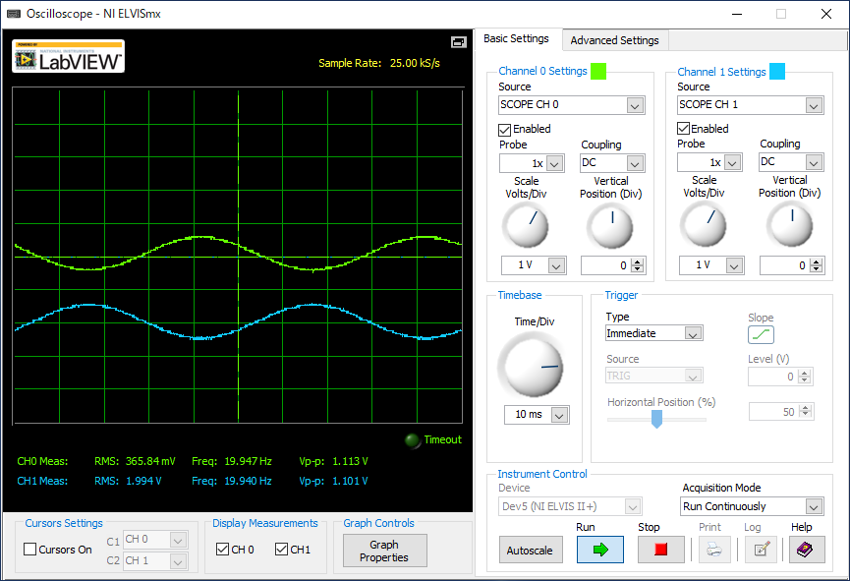
\includegraphics[width=0.8\linewidth]{src/figures/exp7/sum-2.png}
        \subcaption{VPS: \SI{2}{V}}\label{fig:exp7-raw-2}
    \end{subfigure}
    \caption{加算回路の出力波形}\label{fig:exp7-raw}
\end{figure}
